\documentclass[conference]{IEEEtran}
\usepackage{filecontents}
\usepackage[noadjust]{cite}
\usepackage[portuguese]{babel}
\usepackage[utf8]{inputenc}
\usepackage{graphicx}
\usepackage{url}

\begin{filecontents*}{bibi.bib}
	
     @ARTICLE{lee2005tarboard,
   author = {Lee, Wonwoo and Woo, Woontack and Lee, Jongweon},
   title = {Tarboard: Tangible augmented reality system for table-top game environment},
   journal = {2nd International Workshop on Pervasive Gaming Applications, PerGamese},
   year = {2005},
   volume = {5},
   pages = {0-4}
   }
   
   @book{burdea2003virtual,
   	title={Virtual Reality Technology},
   	author={Burdea, G.C. and Coiffet, P.},
   	number={v. 1},
   	isbn={9780471360896},
   	lccn={2002038088},
   	series={Academic Search Complete},
   	year={2003},
   	publisher={Wiley}
   }
   
   @inproceedings{Lam:2006:AAR:1128923.1128987,
   	author = {Lam, Albert H. T. and Chow, Kevin C. H. and Yau, Edward H. H. and Lyu, Michael R.},
   	title = {ART: Augmented Reality Table for Interactive Trading Card Game},
   	booktitle = {Proceedings of the 2006 ACM International Conference on Virtual Reality Continuum and Its Applications},
   	series = {VRCIA '06},
   	year = {2006},
   	isbn = {1-59593-324-7},
   	location = {Hong Kong, China},
   	pages = {357--360},
   	numpages = {4},
   	doi = {10.1145/1128923.1128987},
   	acmid = {1128987},
   	publisher = {ACM},
   	address = {New York, NY, USA},
   	keywords = {augmented reality, card game environment, computer entertainment},
   } 
   
   @inproceedings{Szalavari:1998:CGA:293701.293740,
   	author = {Szalav\'{a}ri, Zsolt and Eckstein, Erik and Gervautz, Michael},
   	title = {Collaborative Gaming in Augmented Reality},
   	booktitle = {Proceedings of the ACM Symposium on Virtual Reality Software and Technology},
   	series = {VRST '98},
   	year = {1998},
   	isbn = {1-58113-019-8},
   	location = {Taipei, Taiwan},
   	pages = {195--204},
   	numpages = {10},
   	doi = {10.1145/293701.293740},
   	acmid = {293740},
   	publisher = {ACM},
   	address = {New York, NY, USA},
   	keywords = {CSCW, augmented reality, interaction, virtual gaming},
   } 
   
   @misc{magic,
   	title = {Magic: The Gathering},
   	howpublished = {\url{http://magic.wizards.com/pt-br}},
   	note = {Accessed: 2015-09-15}
   }
   
   @misc{protour,
   	title = {Magic Origins Pro Tour - Top 8 decklists},
   	howpublished = {\url{http://magic.wizards.com/en/events/coverage/ptori/top-8-decklists-2015-08-01}},
   	note = {Accessed: 2015-11-16}
   }
   
   @misc{magic_duels,
   	title = {Magic Duels},
   	howpublished = {\url{http://magic.wizards.com/content/magic-duels}},
   	note = {Accessed: 2015-09-15}
   }
   
   @misc{3ds,
   	title = {Nintendo AR Games},
   	howpublished = {\url{http://www.nintendo.com/3ds/ar-cards}},
   	note = {Accessed: 2015-11-15}
   }
   
   @misc{unity,
   	title = {Unity - Game Engine},
   	howpublished = {\url{http://unity3d.com/pt/}},
   	note = {Accessed: 2015-09-16}
   }
   
   @misc{eyesony,
   	title = {Sony's The Eye of Judgement},
   	howpublished = {\url{https://en.wikipedia.org/wiki/The_Eye_of_Judgment}},
   	note = {Accessed: 2015-11-15}
   }
   
   @misc{vuforia,
   	title = {Vuforia Developer Portal},
   	howpublished = {\url{https://developer.vuforia.com/}},
   	note = {Accessed: 2015-09-16}
   }
   
   @misc{joao,
   	title = {Artoolkit and Magic the Gathering},
   	howpublished = {\url{https://youtu.be/tpZI1Z-k88Y}},
   	author = {João Batalha},
   	note = {Accessed: 2015-11-16}
   }
   
   @misc{csharp,
   	title = "Guia de Programação em {C}{\#}",
   	howpublished = {\url{https://msdn.microsoft.com/pt-br/library/67ef8sbd.aspx}},
   	note = {Accessed: 2015-09-16}
   }
   
   @misc{magic_cards,
   	title = "MagicCards.info",
   	howpublished = {\url{http://magiccards.info/}},
   	note = {Accessed: 2015-09-16}
   }
\end{filecontents*}

\hyphenation{op-tical net-works semi-conduc-tor}    

\title{Jogo de Cartas Remoto em Realidade Aumentada}

\author{Vítor de Albuquerque Torreão}


\markboth{Disciplina de Realidade Virtual, Setembro~2015}%
{Shell \MakeLowercase{\textit{et al.}}: Bare Demo of IEEEtran.cls for Journals}

\begin{document}
\maketitle

\begin{abstract}
	Os jogos do mundo real e virtual possuem suas próprias vantagens distintas. 
	A realidade aumentada nos permite combinar o melhor dos dois mundos e criar 
	novas formas de jogar. Esta proposta pretende introduzir o ARCGP (Plataforma 
	para jogos de cartas com realidade aumentada). A ideia é prover aos 
	jogadores a experiência dos jogos originais, porém com a possibilidade de 
	jogar remotamente, sem ter de sentar à frente do computador e com baixo 
	custo, sem necessidade de câmeras, mesas vidradas, espelho ou televisores. 
	A plataforma requer apenas um dispositivo capaz de rodar uma aplicação 
	Unity, seja um smartphone ou computador pessoal.
\end{abstract}

\begin{IEEEkeywords}
	Realidade Aumentada, Entretenimento.
\end{IEEEkeywords}

\section{Introdução}
Realidade misturada combina os conteúdos do mundo real com a imaginação virtual.
A realidade aumentada (AR) é um subconjunto da realidade misturada, onde o 
conteúdo digital são sobrepostos aos objetos reais do mundo. Aplicações de 
realidade aumentada suplementam o mundo real com objetos virtuais, de forma que 
o conteúdo gerado pelo computador é adicionado ao ambiente real de forma 
interativa e em tempo real \cite{burdea2003virtual}.

Essas propriedades da realidade aumentada provêm melhorias fascinantes para os 
jogos do mundo real, fazendo-os mais agradáveis e atrativos 
\cite{Lam:2006:AAR:1128923.1128987}. Jogos de cartas são exemplos de jogos que 
podem usufruir das vantagens da Realidade Aumentada. Jogos, como \textit{Magic: 
The Gathering} \cite{magic}, precisam de, no mínimo, dois jogadores, mas não é 
sempre fácil reunir-se com outras pessoas para jogar, de forma que uma 
plataforma que permitisse a dois jogadores disputar uma partida de forma 
remota criaria mais oportunidades de jogo.

Já houveram implementações de \textit{Magic} para computador e dispositivos 
móveis \cite{magic_duels}. No entanto, as plataformas nos quais essas 
aplicações estão disponíveis quebram  a familiaridade do jogador com a forma 
de jogar com a qual está acostumado.

Outras implementações, tais como \cite{joao}, embora mantenham a forma 
tradicional do jogo, necessitam que os dois jogadores estejam no mesmo local 
físico, não os permitindo jogar de forma remota.

A plataforma deveria, então, manter elementos das partidas reais de forma 
que o jogador tivesse a impressão de estar jogando o mesmo jogo, da mesma forma, 
mas eliminar o requisito de deslocamento e compartilhamento do mesmo ambiente 
real.

Portanto, neste artigo será proposta a plataforma ARCGP (\textit{Augmented 
Reality Card Game Platform}). A plataforma consistirá em uma aplicação 
Unity \cite{unity} utilizando a API do Vuforia \cite{vuforia}. 

\subsection{Objetivo}
\label{objetivo}
O objetivo do projeto ARCGP é utilizar o Unity e o Vuforia criar uma plataforma 
de realidade aumentada onde dois jogadores possam disputar uma partida de um 
jogo de cartas sem a necessidade de estarem no mesmo ambiente. ARCGP deve 
reconhecer as cartas em jogo no tabuleiro de um jogador e reproduzi-las através 
de objetos virtuais para o oponente.

O ARCGP deve ser uma plataforma simples, que ocupe pouco espaço físico, que não 
apresente um esforço desnecessário de montagem e que seja de baixo custo.

Como o Vuforia não consegue rastrear mais do que cinco alvos de imagem, serão 
utilizados marcadores. Os jogadores terão de registrar suas cartas previamente, 
momento no qual será feito mapeamento entre as cartas e os identificadores de 
marcadores disponíveis no Vuforia.

Uma imagem será selecionada como alvo para um \textit{extended tracking} 
(rastreamento estendido, em português) e será colocada por cada jogador na sua 
mesa de jogo.

A aplicação deverá ser capaz de se conectar ao dispositivo do adversário. E, a 
partir de então, deverá rastrear os marcadores e exibir para o jogador a imagem 
da carta mapeada no identificador do marcador em questão. Quando este marcador 
for colocado sobre a mesa de jogo, o ARCGP deverá exibir a imagem da carta para 
o jogador, ao mesmo tempo que envia os dados da carta e sua posição em relação 
ao marcador da mesa para o dispositivo do adversário, que irá, por sua vez, 
transladar e rotacionar a carta para exibi-la corretamente.

Este artigo está estruturado da seguinte forma: na seção \ref{rel} serão 
apresentados trabalhos relacionados; na seção \ref{metodologia} será 
apresentada a metodologia utilizada no desenvolvimento da plataforma; na 
seção \ref{plataforma}, a plataforma propriamente dita será apresentada em 
detalhes; em seguida, a seção \ref{conclusao} trás algumas considerações finais 
sobre o projeto; por fim, a seção \ref{trab_fut} trás alguns trabalhos futuros 
para serem realizados em cima da ARCGP.

\section{Trabalhos Relacionados}
\label{rel}
Utilizar realidade aumentada em jogos eletrônicos não é novidade. Isso vem sendo 
feito nos \textit{consoles} e portáteis da Sony e da Nintendo, por exemplo.

Por parte da Sony se tem o \textit{Eye of Judgement} \cite{eyesony}, para 
\textit{Playstation 3}, que se trata de um jogo de cartas original criado pela 
produtora. O jogo se vale do \textit{Playstation Eye} para capturar a cena real 
e utiliza o próprio console para fazer os cálculos de rastreamento. Os jogadores 
podem jogar de forma remota, online, ou em um \textit{multiplayer} presencial. 
Deve-se notar que não é possível jogar outros jogos de cartas com esse recurso.

Já a Nintendo lançou o \textit{AR Games} \cite{3ds} que é uma compilação de 
mini-jogos e ferramentas simples que vêm pré-instaladas no portátil Nintendo 
3DS. Junto vêm seis cartas, cinco delas com os principais personagens da 
produtora e uma com uma interrogação. Essas cartas podem ser utilizadas por 
diferentes jogos para incrementar a experiência do usuário.

Outros trabalhos realizados envolvendo jogos de cartas com realidade aumentada 
trabalham em cima do cenário onde dois jogadores estão no mesmo ambiente e focam 
trazer a imaginação do jogador para a realidade através da sobreposição de 
objetos virtuais. As plataformas propostas, no entanto, requerem um hardware 
específico e, muitas vezes, de alto custo.

O desenvolvedor João Batalha implementou uma aplicação de realidade aumentada 
capaz de permitir a dois jogadores jogarem uma partida do jogo \textit{Magic: 
The Gathering}. A aplicação checa se as jogadas são permitidas pela regra, 
controla os turnos do jogo e exibe gráficos 3D dos personagens de cada carta 
como um objeto virtual sobreposto à cena real. No entanto, a aplicação necessita 
que os jogadores estejam no mesmo local físico \cite{joao}.

Em \cite{Szalavari:1998:CGA:293701.293740}, os pesquisadores montaram um sistema 
de realidade aumentada para jogadores compartilharem um ambiente virtual onde 
jogam \textit{Mah-Jongg}. Os objetivos do sistema desenvolvido por eles é 
aplicar realidade aumentada para melhorar a experiência do usuário mantendo os 
aspectos da interação social e privacidade. O sistema consiste de um 
\textit{head mounted display} (HMD) e um painel de interação pessoal para cada 
jogador, além de um servidor que roda a simulação do jogo. O HMD não bloqueia 
totalmente a visão do ambiente, permitindo a um jogador se comunicar com o outro 
através de gestos, e os elementos virtuais exibidos no HMD permitem que cada 
usuário tenho uma visão diferente do jogo, garantindo a privacidade.

Assim, \cite{Szalavari:1998:CGA:293701.293740} apresenta um sistema com uma 
aplicação diferente da plataforma proposta neste artigo já que ele visa simular 
um jogo de mesa e exibi-lo aos jogadores por meio de realidade aumentada, 
enquanto que neste projeto a realidade aumentada é utilizada para permitir que 
jogadores distantes possam jogar como se estivessem no mesmo ambiente, sem 
necessidade de simular o jogo em computador.

O TARBoard \cite{lee2005tarboard} é um sistema que utiliza a realidade aumentada 
e a interface de usuário tangível para melhorar a experiência do usuário nos 
jogos de cartas e de tabuleiro em geral. O TARBoard consiste de uma mesa de 
vidro, duas câmeras e um espelho. Marcadores são colocados embaixo dos objetos 
e/ou cartas do jogo. Uma das câmeras fica posicionada embaixo da mesa e rastreia 
os marcadores. A segunda câmera provê imagens para aumentar os objetos virtuais. 
Os usuários veem os objetos virtuais no \textit{stream} de vídeo das câmeras.

O objetivo do TARBoard é bem diferente do ARCGP, pois ele pretende melhorar a 
experiência tradicional do jogo sem, no entanto, substituí-la como o ARCGP.

O ART (\textit{Augmented Reality Table}) \cite{Lam:2006:AAR:1128923.1128987} é 
uma plataforma que usa a tecnologia da realidade aumentada para prover uma mesa 
virtual para os jogadores. Ela consiste de um computador, um monitor e uma 
câmera. A câmara, que é o único dispositivo de entrada do sistema, fica 
posicionada acima dos jogadores e captura os eventos da mesa. O monitor fica 
posicionado na horizontal servindo como mesa para os jogadores, que jogam de 
forma natural e tradicional. Este monitor exibe para os jogadores o ambiente 
virtual com som e imagem aumentados. O computador é a unidade de processamento 
do sistema, capturando as imagens, reconhecendo as entradas válidas e produzindo 
as saídas correspondentes de acordo com as regras do jogo.

É importante observar algumas limitações do ART. Primeiramente, é necessário 
que os jogadores estejam no mesmo ambiente. Além disso, é necessário montar 
toda uma estrutura de hardware para o correto funcionamento da plataforma: 
posicionar a câmera de forma a capturar os eventos da mesa, posicionar o monitor 
corretamente e conectar ambos ao computador. Por fim, esses equipamentos 
possuem um custo elevado para os jogadores.

\section{Metodologia}
\label{metodologia}
Para desenvolver essa plataforma será utilizado o jogo \textit{Magic: The 
Gathering} como exemplo, por se tratar de um jogo baseado em turnos e onde 
o requisito de tempo real não é muito importante: atrasos de até alguns segundos 
não atrapalham a jogabilidade do jogo. 

Primeiramente, foi realizado um estudo aprofundado do Unity, da linguagem de 
programação C\# \cite{csharp} e do Vuforia. Após essa etapa, foi elaborada a 
arquitetura necessária para tornar a aplicação viável.

Em seguida, foi necessário criar um banco de dados para testes com algumas 
cartas. Existem diversos \textit{websites} que disponibilizam imagens de cartas, 
como por exemplo, \cite{magic_cards}. Foram montados dois \textit{decks} para 
os testes, ambos oriundos do \textit{Pro Tour Magic Origins}. Foram 
selecionados os \textit{decks} do campeão e do vice, Joel Larsson e Mike Sigrist 
\cite{protour}.

Depois, a aplicação propriamente dita foi desenvolvida utilizando as ferramentas 
mencionadas e de acordo com os requisitos explanados na seção \ref{objetivo}.
O primeiro passo para o desenvolvimento da aplicação foi o desenvolvimento de 
um \textit{script} C\# que preparasse as instâncias da aplicação para se 
conectarem e trocarem mensagens. O segundo foi a preparação de um outro 
\textit{script}, novamente na linguagem C\#, que modificasse a cena adicionando 
os \textit{frame markers} e suas respectivas cartas em tempo de execução, 
fazendo a leitura do arquivo de configuração contendo a lista de cartas que 
compõem o \textit{deck} do jogador. O terceiro passo foi o desenvolvimento do 
esquema de comunicação para que uma instância comunicasse a outra quais cartas 
foram colocadas em jogo pelo seu jogador e quais cartas foram removidas de jogo.

No decorrer e após essa etapa, foram feitos diversos testes com dois jogadores 
para verificar a funcionalidade da ferramenta e se os requisitos foram 
satisfeitos.

Por fim, a ferramenta foi apresentada à comunidade através da redação deste 
artigo e de uma apresentação realizada na Universidade Federal Rural de 
Pernambuco.

\section{A plataforma}
\label{plataforma}
A atual implementação do ARCGP é uma aplicação que se vale da plataforma Unity 
\cite{unity} para toda a parte da gerência da cena e dos objetos 3D, além da 
comunicação com os dispositivos dos jogadores adversários. Ela também utiliza a 
API do Vuforia \cite{vuforia} para a parte de Realidade Aumentada. O Vuforia é 
um \textit{kit} de desenvolvimento de aplicações de realidade aumentada 
disponível para diferentes plataformas, inclusive para o Unity através de  um 
plugin.

A ARCGP é dividida entre dois principais componentes: a cena 3D e os 
\textit{scripts} de comportamento.

\subsection{Cena 3D}
\label{cena3d}
A cena 3D pode ser descrita através da hierarquia montada no Unity. Essa 
hierarquia está ilustrada na Figura \ref{hierarchy}.

\begin{figure}[t]
	\caption{Hierarquia da Cena 3D tal como foi montada no Unity 3D}
	\label{hierarchy}
	\centering
	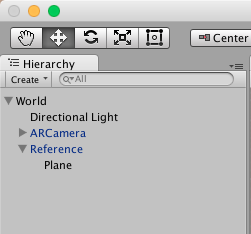
\includegraphics[width=0.25\textwidth]{hierarchy}
\end{figure}

O primeiro elemento, \textit{World}, do qual todos os outros são filhos, é o 
responsável por conter dois \textit{scripts} de comportamentos específicos da 
aplicação. Um deles é o \textit{LoadDeck.cs} que fica responsável por ler o 
arquivo de configuração e preparar sessenta \textit{frame markers} com as cartas 
do jogador. O outro é o \textit{Configuration.cs} responsável por carregar todo 
tipo de configuração que possa ser alterada pelo jogador antes de executar a 
aplicação. Por exemplo, o endereço na internet, IP, do adversário é carregado 
por este \textit{script}.

O segundo elemento, a \textit{Directional Light}, é um objeto que vem por padrão 
nas cenas assim que o Unity as cria. Nenhuma configuração adicional foi feita 
neste objeto.

O terceiro elemento, a \textit{AR Camera}, é um \textit{prefab} importado do 
Vuforia. Nele foi configurada a \textit{API Key} da aplicação. Sem esta 
informação, a ARCGP não seria capaz de utilizar a biblioteca de Realidade 
Aumentada. Também neste objeto está o \textit{script} de comportamento \textit{
NetworkEnvironmentShare.cs}. Ele é responsável por toda a parte de comunicação 
e rede da aplicação. Esse \textit{script} será detalhado na seção seguinte.

Por fim, tem-se o objeto chamado de \textit{Reference}. Esse pode ser chamado de 
um objeto coringa, pois no seu lugar pode-se ser colocado qualquer \textit{
prefab} rastreável desde que se substitua o \textit{script} de comportamento 
\textit{DefaultTrackableEventHandler.cs}, que é padrão da biblioteca Vuforia, 
pelo \textit{script ReferenceEnvironmentTracker.cs}. O comportamento que esse 
\textit{script} está responsável por enforçar será detalhado na seção seguinte.

No exemplo testado, foi utilizado um alvo de marcador comum, mas o usuário pode 
alterar esse objeto colocando um \textit{Image Target prefab} e utilizar uma 
imagem de sua escolha e possibilitar um \textit{extended tracking}, por exemplo.

\subsection{\textit{Scripts} de comportamento}
\label{scripts}
Foram preparados cinco \textit{scripts}, na linguagem C\# para implementar as 
funcionalidades previstas pelo projeto da ARCGP. Estes serão descritos em 
detalhes nesta seção.

\section{Conclusão}
\label{conclusao}
Neste artigo, foi descrito o projeto da Plataforma para Jogos de Cartas com 
Realidade Aumentada. Foram explicitados seus objetivos, metodologia, resultados 
esperados e o cronograma para conclusão do projeto.

Além disso, foram levantados alguns trabalhos com matérias parecidas e foram 
esclarecidas as diferentes entre eles e o ARCGP.

\section{Trabalhos Futuros}
\label{trab_fut}
Aqui são apresentados alguns trabalhos.

\bibliographystyle{IEEEtran}
\bibliography{bibi}
\end{document}